\let\textcircled=\pgftextcircled
\chapter{Sensory Apparatus}
\label{chap:sensors}

\initial{S}ome data will be obtained from sources external to this project such as the GPS and the stereo camera disparity map. Additional sensors must be chosen to augment these incoming data sources and to cover as many blind spots as possible in the drones perception of the environment. The data required is largely based around range finding and drone movement to aid with collision avoidance. 

%=======

\section{Sensor Basics}
\label{sec:sensorbasics}
Sensors come in two basic forms, active and passive. Active sensors require a signal to be generated by the apparatus that is later detected by a receiver, a good example of this would be a RADAR system which emits radio waves then detects the reflections. Passive sensors receive signals solely generated by the environment, such as heat detected by a thermal camera. The two forms have contrasting pros and cons. Active sensors are generally more accurate and less sensitive to noise, however this comes at the cost of significantly higher energy consumption. Passive sensors are correspondingly very low power, however they rely on the environment to provide usable signal at all times. They do allow "silent running", meaning that their use cannot be detected by a third party. \par
	While it would be ideal for the drone to make full use of low power passive sensors, the range finding data required is difficult to obtain through passive methods, relying for instance on expensive stereo cameras. Though the drone will have one stereo camera aboard, it is not financially viable to have multiple units facing in all directions. For this reason the stereo camera will be mounted forwards facing, and much cheaper sensors will be utilised elsewhere.

\section{Sensor Experimentation}
\label{sec:sensorexperimentation}
There are a few sensors that can obtain the ranging data required, each with strengths and weaknesses.\par
\begin{itemize}
\item Ultrasonic time-of-flight, active: These sensors have a conical detection pattern that allows detection of a fairly wide area but at the cost of spatial resolution, figure \ref{fig:ultrasonicdiagram} shows the basic function. Range and depth accuracy is variable with the quality of the sensor, but is typically around 5 cm to 4 m with 1 cm resolution. Polling rate for this sensor is limited  by the speed of sound; for a sensor rated to 2 m the theoretical minimum time between readings is given by the travel time to and back from maximum distance, in this case \((2\; m \times 2) \div 343\; ms^{-1} = 12\; milliseconds\) and hence polling rate of \(1/12\; milliseconds = 86\; Hz\). There are also certain conditions that can affect the operation of the sensor. Temperature will affect air density and hence the speed of sound meaning that calibration must be performed to ensure accurate readings. The reflective surface must be perpendicular to the sensor for the sound waves to bounce back to the receiver, deviation from this angle will drastically reduce signal return. The degree to which the surface absorbs sound can cause objects at the range extremities to not be detected, and makes it infeasible to use received power as a distance estimator outside of a calibrated, controlled environment, leaving time of flight as the only realistic range finding method. Advanced receivers can however determine whether a detected object is moving away from or towards the receiver based on Doppler shift \cite{petrescu2012new}.


\begin{figure}[h]
	\centering
	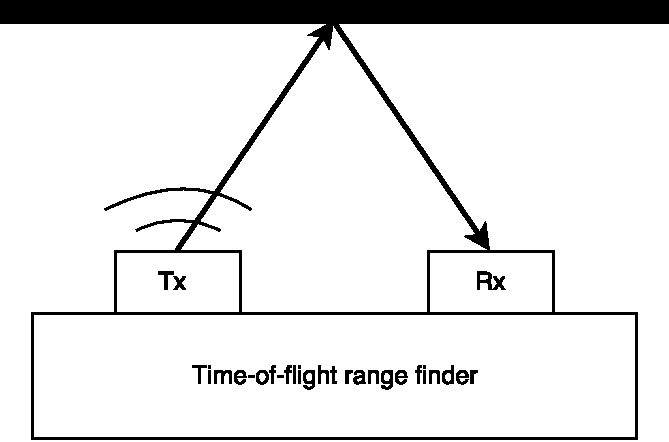
\includegraphics[height=0.25\textheight]{ultrasonic.pdf}
	\mycaption[Time-of-Flight Range Finder Diagram]{Diagram showing the basic mechanism behind a time-of-flight range finder}
	\label{fig:ultrasonicdiagram}
\end{figure}

\item Laser time-of-flight, active: While being fairly similar to the ultrasonic time-of-flight sensors, the laser has a much tighter conical detection pattern, a maximum of about 5\textsuperscript{o}, and a much faster signal travel speed resulting in higher possible polling rates. However it generally has a lower detection range due to the higher passive environmental noise and the tighter beam has a higher tolerance on reflection angle. Their power level is also fairly limited due to needing to make them eye-safe.

\item LiDAR, active: An extension of laser time-of-flight, LiDAR (\underline{Li}ght \underline{D}etection \underline{a}nd \underline{R}anging) usually utilises a single laser to produce a two or three dimensional point cloud by rapidly sweeping the laser and taking measurements at various angles \cite{lidaruk2017how}\cite{cracknell2007introduction}. This apparatus is often used for topographical mapping from aircraft \cite{Nayegandhi2006green}. The technique greatly increases the complexity of the receiving equipment however as rotation of the measure point must be accounted for and inter-point interference should be minimised. A similar but much less applicable technology SoDAR uses the same principles but with ultrasonics, mostly utilised to measure atmospheric turbulence.
%LiDAR diagram

\item Pressure altimeter, passive: Pressure altimeters are cheap but reliable sensors with very low weight and power consumption. They are affected by varying atmospheric pressure caused by  moving weather systems however are fairly immune to value drifting otherwise.		
\end{itemize}

LiDAR would clearly be the most ideal for this project due to its ability to rapidly scan a full  360\textsuperscript{o} using the arguably superior laser time-of-flight sensor. However, even a relatively cheap two dimensional LiDAR unit weighs 340g, a not insignificant amount of weight for a drone to carry, and more crucially costs over \pounds 400 which is not fiscally viable for this project \cite{slamtec2016rplidar}. The best alternative seems to be using a mixture of ultrasonic and laser time-of-flight sensors with one or two pressure altimeters for height. The ultrasonic sensors are very cheaply available \cite{amazon2017ultrasonics} with the laser sensors a bit more expensive but still feasible. These readings can then be mixed to provide a better value estimate than would be achieved from each independently.


\section{Implemented Sensory Apparatus}
The final sensory array for the drone was not fully assembled however the general layout was proposed and can be seen in figure \ref{fig:sensordiagram}.

\subsection{Proposed Layout}
\begin{itemize}
\item One ultrasonic time-of-flight range finder facing up, down, and at each cardinal direction.
\item One laser time-of-flight range finder facing up, down, and at each cardinal direction.
\item One disparity mapped stereo camera facing forwards.
\item One barometer.
\item One global positioning system unit.
\item Two inertial measurement units.
\end{itemize}

\begin{figure}[ht]
	\centering
	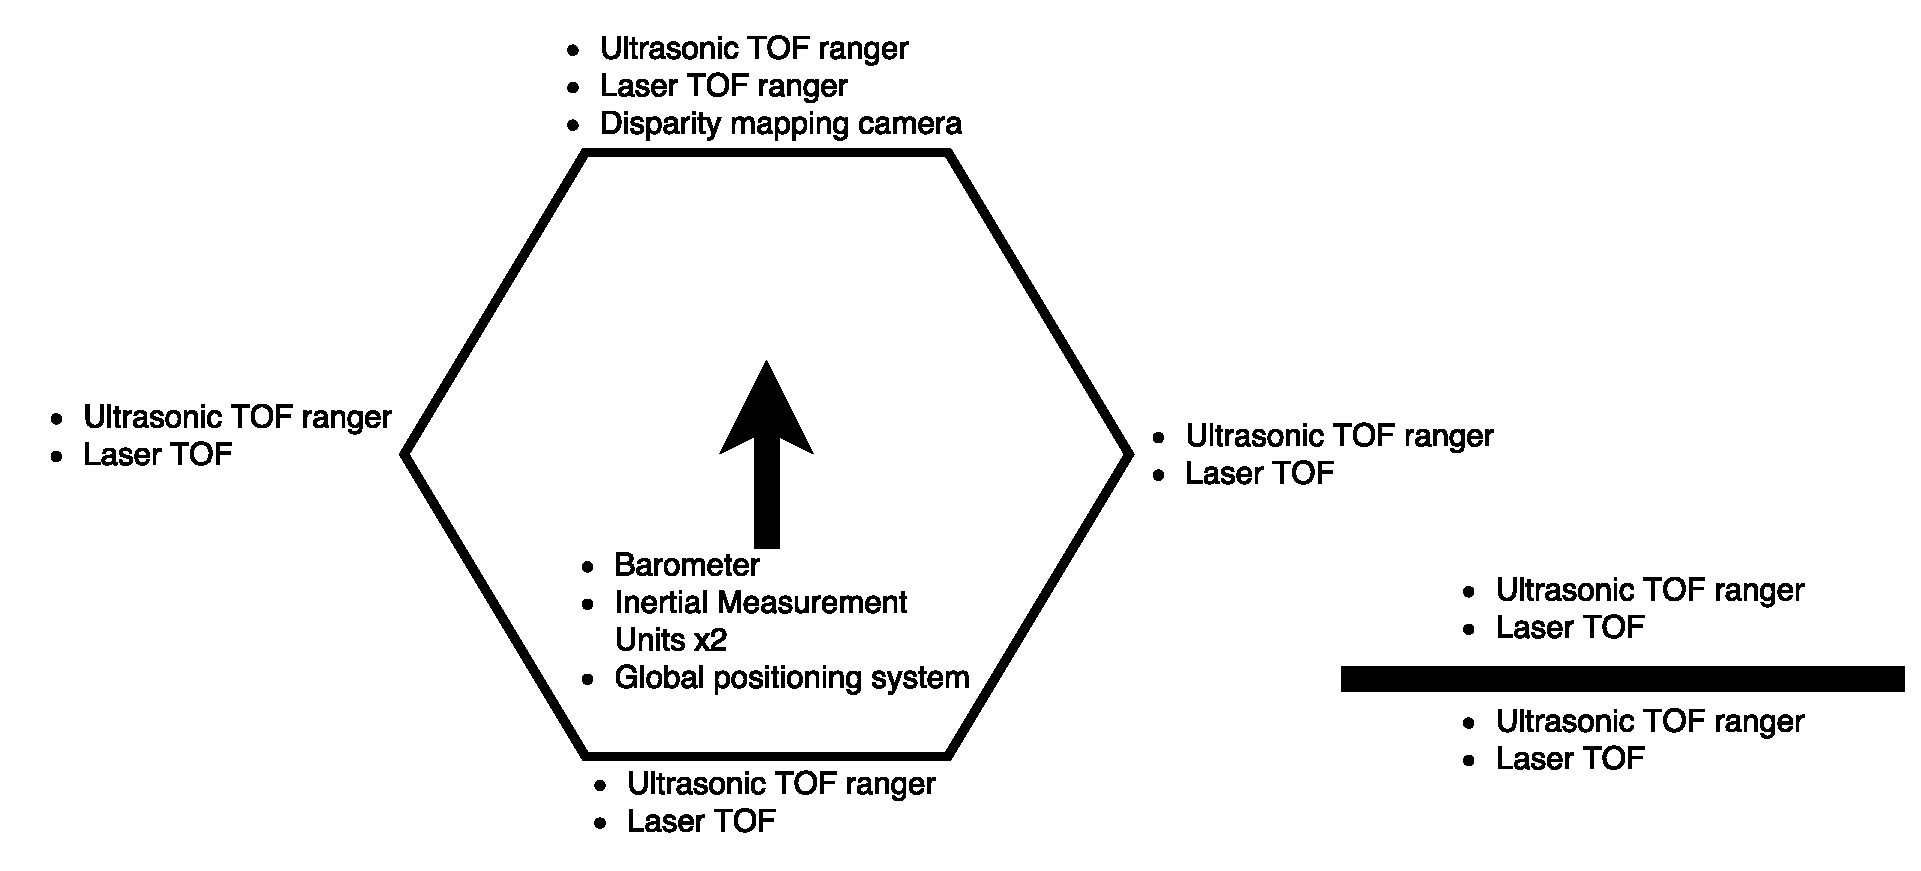
\includegraphics[width=\textwidth]{sensordiagram.pdf}
	\mycaption[Drone's Sensor Apparatus Diagram]{Diagram showing top-down (left) and front (right) views of the drone indicating where sensory apparatus has been placed.}
	\label{fig:sensordiagram}
\end{figure}

This will provide ample data to work on as well as redundancy in the case of failure of one of the sensors.


\subsection{Sensor Characterisation}
Sensor characterisation was achieved through data sheet information except for the disparity mapping which was done manually by the project focusing on it.
Table \ref{tab:sensors} gives sensor characteristics.

\begin{table}[ht]
\centering
\begin{tabular}{@{}lllll@{}}
\toprule
\textbf{Sensor}             & \textbf{Units} & \textbf{Min. Range} & \textbf{Max Range} & \textbf{Sensor Variance} \\ \midrule
Ultrasonic time-of-flight \cite{HCSR04datasheet}   & \textit{cm}    & 2                   & 400                & 4                        \\
Laser time-of-flight \cite{VL53L0Xdatasheet}       & \textit{cm}    & 0                   & 120                & 1                        \\
Stereo camera disparity Map & \textit{cm}    & 10                  & 5500               & 10                       \\
Barometer \cite{MS5611datasheet}                  & \textit{mbar}  & 10                  & 1200               & 3                        \\
Global positioning system \cite{NEO6Mdatasheet}   & \textit{m}     & N/A                 & N/A   & 2                       \\ 
Inertial measurement unit (1) \cite{L3GD20datasheet}   & \textit{o}   & N/A                 & N/A                & 8.75                     \\
Inertial measurement unit (2) \cite{MPU9250datasheet}   & \textit{o}   & N/A                 & N/A                & 5                     \\ \bottomrule
\end{tabular}
\caption{Sensor characteristics}
\label{tab:sensors}
\end{table}

The camera used was the Tara - USB 3.0 Stereo Vision Camera made by e-con Systems \cite{econ2016tara}. Though versatile it is too expensive to have more than one.







